%%%
%
% $Autor: Nayan $
% $Date: 2024-10-31 11:15:45Z $
% $File: file.tex $
% $Version: 1 $
%
% Project: 
%
%%%

\chapter{Statsmodels}
\label{ch:statsmodels}

\section{Introduction}

\textbf{Statsmodels} is the main statistical modeling library used in this project. While \textbf{scikit-learn} is used for evaluation metrics and \textbf{Streamlit} is used for the dashboard, \textbf{statsmodels} is the package that actually estimates the forecasting models discussed in this report. In practical terms, it is the library behind the ARIMA, ETS, and SARIMA implementations used for Germany's monthly CPI series.

This makes the package academically important for the report. The quality of the forecasting comparison depends not only on the selected models, but also on whether those models are implemented in a statistically appropriate and reproducible way. \textbf{Statsmodels} is a good fit for this purpose because it provides mature time-series classes, support for prediction intervals, and a workflow that integrates naturally with \textbf{pandas} time indices \cite{Box2015,Hyndman2021,statsmodels-doc}.

\section{Description}

The most relevant \textbf{statsmodels} components for this repository are the time-series classes imported in \FILELOC{Code/src/models.py}:

\begin{itemize}
    \item \texttt{statsmodels.tsa.arima.model.ARIMA}
    \item \texttt{statsmodels.tsa.exponential\_smoothing.ets.ETSModel}
    \item \texttt{statsmodels.tsa.statespace.sarimax.SARIMAX}
\end{itemize}

These classes are wrapped inside project-specific Python classes so that all forecasting models share a consistent interface with \texttt{fit()}, \texttt{predict()}, and \texttt{get\_confidence\_intervals()} methods. This wrapper design matters because it allows the modeling pipeline in \FILELOC{Code/src/modeling\_pipeline.py} to train, forecast, evaluate, and serialize different models with the same control logic rather than handling each one separately.

Statsmodels is also used indirectly during exploratory analysis. The EDA pipeline relies on functions such as the Augmented Dickey-Fuller test and seasonal decomposition tools, both of which help justify later model choices in a methodologically transparent way.

Table~\ref{tab:statsmodels-project-mapping} summarizes the most important \textbf{statsmodels} classes used in the repository.

\begin{table}[htbp]
    \centering
    \caption{Mapping of statsmodels classes to project use.}
    \label{tab:statsmodels-project-mapping}
    {\small
    \renewcommand{\arraystretch}{1.22}
    \setlength{\tabcolsep}{7pt}
    \begin{tabular}{L{4.1cm}L{8.5cm}}
        \hline
        Statsmodels class & Project use \\
        \hline
        \texttt{ARIMA} & Non-seasonal baseline forecasting model for autocorrelation-driven CPI prediction \\
        \texttt{ETSModel} & State-space exponential-smoothing model for level, trend, and seasonal structure \\
        \texttt{SARIMAX} & Seasonal forecasting model used to implement SARIMA with monthly seasonality \\
        \hline
    \end{tabular}
    }
\end{table}

\section{Installation}

\textbf{Statsmodels} is listed in \FILELOC{Code/requirements.txt} and is normally installed together with the full project environment:

\begin{Python}[caption={Installing project dependencies including statsmodels}, label={lst:install_statsmodels_project}]
pip install -r Code/requirements.txt
\end{Python}

If a separate installation is needed, the direct command is:

\begin{Python}[caption={Installing statsmodels directly}, label={lst:install_statsmodels_direct}]
pip install statsmodels
\end{Python}

The installation can be verified as follows:

\begin{Python}[caption={Verifying the statsmodels installation}, label={lst:verify_statsmodels}]
import statsmodels
print(statsmodels.__version__)
\end{Python}

\section{Example -- Description}

A repository-specific example is the definition of the three forecasting wrappers in \FILELOC{Code/src/models.py}. The project does not call raw \textbf{statsmodels} classes directly from the dashboard or the evaluation loop. Instead, it places them behind a common interface so that ARIMA, ETS, and SARIMA can be used interchangeably during training and prediction.

This is a useful engineering decision. It keeps the statistical strengths of statsmodels while reducing repetition in the application code. It also makes the evaluation stage easier to document and easier to trust, because the forecasting pipeline can loop over models without introducing separate control branches for each class.

\section{Example -- Manual}

The practical use of statsmodels in this project can be reproduced through the following steps:

\begin{enumerate}
    \item Install the project dependencies.
    \item Load the cleaned CPI series using \FILELOC{Code/src/data\_loader.py}.
    \item Instantiate the model wrappers defined in \FILELOC{Code/src/models.py}.
    \item Fit the models on the training portion of the CPI series.
    \item Generate 24-step forecasts and, where available, prediction intervals.
    \item Compare results in \FILELOC{Code/src/modeling\_pipeline.py} and reuse the trained objects in \FILELOC{Code/app.py}.
\end{enumerate}

\section{Example -- Code}

Listing~\ref{lst:statsmodels_project_code} shows the core form of statsmodels usage employed by the project.

\begin{Python}[caption={Project-specific statsmodels model definitions}, label={lst:statsmodels_project_code}]
from statsmodels.tsa.arima.model import ARIMA
from statsmodels.tsa.exponential_smoothing.ets import ETSModel
from statsmodels.tsa.statespace.sarimax import SARIMAX

model_arima = ARIMA(train_series, order=(1, 1, 1))
model_ets = ETSModel(train_series, error='add', trend='add', seasonal='add', seasonal_periods=12)
model_sarima = SARIMAX(train_series, order=(1, 1, 1), seasonal_order=(1, 1, 1, 12))
\end{Python}

In the repository, these calls are embedded in wrapper classes in \FILELOC{Code/src/models.py} so that the forecasting pipeline can handle them uniformly. This gives the project a clearer separation between statistical modeling and application logic.

\section{Example -- Files}

The most important files in which statsmodels appears are:

\begin{itemize}
    \item \FILELOC{Code/src/models.py} -- imports and wraps ARIMA, ETSModel, and SARIMAX.
    \item \FILELOC{Code/src/modeling\_pipeline.py} -- fits wrapped models, generates forecasts, and saves artifacts.
    \item \FILELOC{Code/src/eda\_pipeline.py} -- uses statsmodels-based diagnostics such as ADF testing and seasonal decomposition.
    \item \FILELOC{Code/app.py} -- consumes trained statsmodels-based wrappers after serialization.
\end{itemize}

\section{Package Role in the CPI Pipeline}

The following figure is not intended to replace the global KDD methodology in Chapter~\ref{ch:kdd-methodology}. Instead, it zooms in on the \textbf{data-mining stage} and shows the specific role of \textbf{statsmodels} inside the implemented forecasting pipeline. In this project, the package receives the cleaned CPI series after selection, preprocessing, and transformation have already been completed. It then provides the statistical model classes for ARIMA, ETS, and SARIMA, which are wrapped in the repository code, fitted to the series, and used to generate forecasts together with confidence intervals. The figure therefore gives a smaller package-level view nested inside the broader KDD process.

\begin{figure}[htbp]
\centering
\resizebox{0.95\linewidth}{!}{
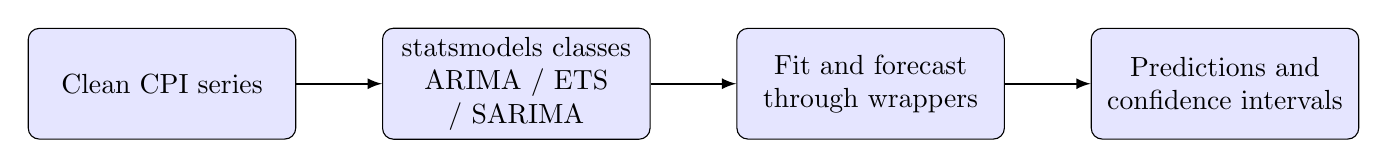
\begin{tikzpicture}[
    block/.style={rectangle, draw, fill=blue!10, text width=9em, text centered, rounded corners, minimum height=4em},
    line/.style={draw, -latex, thick}
]
    \node [block] (series) at (0,0) {Clean CPI series};
    \node [block] (models) at (4.5,0) {statsmodels classes\\ARIMA / ETS / SARIMA};
    \node [block] (fit) at (9,0) {Fit and forecast\\through wrappers};
    \node [block] (out) at (13.5,0) {Predictions and\\confidence intervals};

    \draw [line] (series) -- (models);
    \draw [line] (models) -- (fit);
    \draw [line] (fit) -- (out);
\end{tikzpicture}
}
\caption{Package-level view of \textbf{statsmodels} within the CPI pipeline. In KDD terms, the figure corresponds primarily to the data-mining stage, where the cleaned and transformed CPI series is passed to the forecasting models, fitted through repository wrappers, and converted into predictions with confidence intervals.}
\label{fig:statsmodels_workflow}
\end{figure}

\section{Further Reading}

\begin{itemize}
    \item Statsmodels documentation: \URL{https://www.statsmodels.org/}
    \item Time-series user guide: \URL{https://www.statsmodels.org/stable/tsa.html}
    \item Hyndman and Athanasopoulos, \textit{Forecasting: Principles and Practice} \cite{Hyndman2021}
    \item Box, Jenkins, Reinsel, and Ljung, \textit{Time Series Analysis: Forecasting and Control} \cite{Box2015}
\end{itemize}
